\documentclass[leqno]{article}
\usepackage[utf8]{inputenc}
\usepackage[T1]{fontenc}
\usepackage{amsfonts}
\usepackage{fourier}
\usepackage{heuristica}
\usepackage{enumerate}
\author{Colin Roberts}
\title{MATH 560, Cats, Dogs, and the SVD}
\usepackage[left=3cm,right=3cm,top=3cm,bottom=3cm]{geometry}
\usepackage{amsmath}
\usepackage[thmmarks, amsmath, thref]{ntheorem}
%\usepackage{kbordermatrix}
\usepackage{mathtools}

\usepackage{tikz-cd}

\theoremstyle{nonumberplain}
\theoremheaderfont{\itshape}
\theorembodyfont{\upshape:}
\theoremseparator{.}
\theoremsymbol{\ensuremath{\square}}
\newtheorem{proof}{Proof}
\theoremsymbol{\ensuremath{\square}}
\newtheorem{lemma}{Lemma}
\theoremsymbol{\ensuremath{\blacksquare}}
\newtheorem{solution}{Solution}
\theoremseparator{. ---}
\theoremsymbol{\mbox{\texttt{;o)}}}
\newtheorem{varsol}{Solution (variant)}

%%Matlab packages stuff
\usepackage[framed,numbered,autolinebreaks,useliterate]{mcode}

\newcommand{\tr}{\mathrm{tr}}
\newcommand{\R}{\mathbb{R}}
\newcommand{\F}{\mathbb{F}}

\begin{document}
\maketitle
\begin{large}
\begin{center}
Solutions
\end{center}
\end{large}
\pagebreak

%%%%%%%%%%%%%%%%%%%%%%%%%%%%%%%%%%%%%%%%%%%%%%%%%%%%%%%%%%%%%%%%%%%%%%%%%%%%%%%%%%%%%%%%%%%%%%%%%%%%%%%%%%%%%%%%%%%%%
%%%%%%%%%%%%%%%%%%%%%%%%%PROBLEM%%%%%%%%%%%%%%%%%%%%%%%%%%%%%%%%%%%%%%%%%%%%%%%%%%%%%%%%%%%%%%%%%%%%%%%%%%%%%%%%%%%%%%%%%%%%%%%%%%%%%%%%%%%%%%%%%%%%%%%%%%%%%%%%%%%%%%%%%%%%%%%%%%%%%%%%%%%%%%%%%%%%%%%%%%%%%%%%%%%%%%%%%%%%%%%%%%%%%%%%%%
\noindent\textbf{Problem 1.} \\

We wish to calculuate the singular value decomposition for a matrix.  In this case, our matrices $C$ and $D$ are formed by turning $64\times 64$ grayscale images of cats and dogs into vectors of length $4096$ and appending them as columns into the matrices $C$ and $D$ respectively.  

Of course, we will calculate the singular value decomposition as follows.  Using the form $A=U\Sigma V^T$ we form the matrices,

\begin{align*}
C&= U_{cat} S_{cat} V_{cat}^T\\
D&= U_{dog} S_{dog} V_{dog}^T. 
\end{align*}
In this case, $U_{cat}U_{cat}^T=I_{4096\times 4096}=U_{dog}U_{dog}^T$ and $V_{cat}V_{cat}^T=I_{64\times 64}=V_{dog}V_{dog}^T$ as well as $S_{cat}$ and $S_{dog}$ are $4096\times 64$ matrices with singular values along the diagonal, and all other values zero.  The first column of $U_{cat}$ and of $U_{dog}$ will be the first left singular values of the matrices $C$ and $D$ respectively and it's worth noting that these vectors correspond to the largest singular values.

\begin{lstlisting}
%Calculate the left singular Cat vectors
[U_cat,S_cat,V_cat] = svd(C);
%Display the first singular Cat vector
imagesc(reshape(U_cat(:,1),64,64))
\end{lstlisting}

In order to view the first left singular vectors, we must reshape the vectors from $4096\times 1$ to $64\times 64$.  This is done in the last line here, and we have the following image.

\begin{figure}[h]
\begin{center}
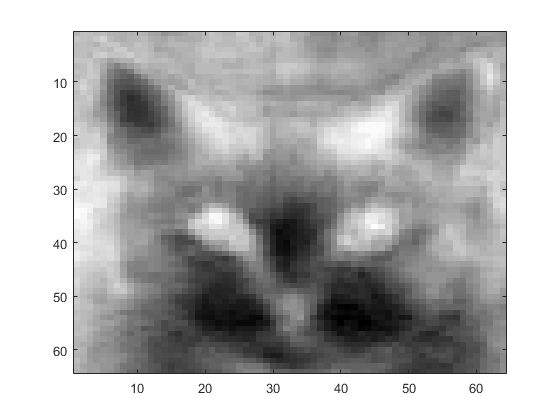
\includegraphics[scale=.4]{left_singular_cat.png}
\caption{The first left singular cat vector.}
\end{center}
\end{figure}


\begin{lstlisting}
%Calculate the left singular Dog vectors
[U_dog,S_dog,V_dog]=svd(D);
%Display the first singular Dog vector
imagesc(reshape(U_dog(:,1),64,64))
\end{lstlisting}

\begin{figure}[h]
\begin{center}
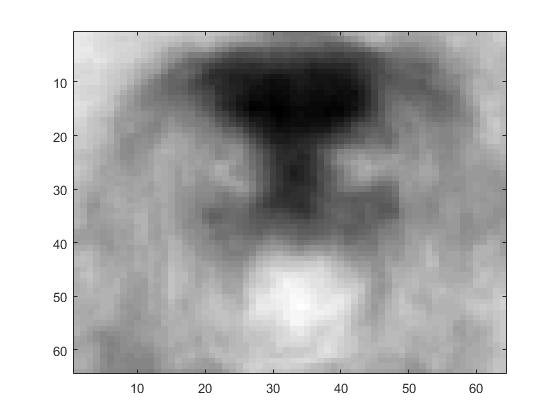
\includegraphics[scale=.4]{left_singular_dog.png}
\caption{The first left singular dog vector.}
\end{center}
\end{figure}

\pagebreak

%%%%%%%%%%%%%%%%%%%%%%%%%%%%%%%%%%%%%%%%%%%%%%%%%%%%%%%%%%%%%%%%%%%%%%%%%%%%%%%%%%%%%%%%%%%%%%%%%%%%%%%%%%%%%%%%%%%%%
%%%%%%%%%%%%%%%%%%%%%%%%%PROBLEM%%%%%%%%%%%%%%%%%%%%%%%%%%%%%%%%%%%%%%%%%%%%%%%%%%%%%%%%%%%%%%%%%%%%%%%%%%%%%%%%%%%%%%%%%%%%%%%%%%%%%%%%%%%%%%%%%%%%%%%%%%%%%%%%%%%%%%%%%%%%%%%%%%%%%%%%%%%%%%%%%%%%%%%%%%%%%%%%%%%%%%%%%%%%%%%%%%%%%%%%%%


\noindent\textbf{Problem 2.} \\
Now we want to see how we can represent a cat by using the dog basis found from the SVD and do the same for a dog using the cat basis found from the SVD.  In order to do this, we just use the following idea:
\begin{align*}
w_{cat}&=\sum_{i=1}^{99} \langle C_1, U_{{dog}_i} \rangle U_{{dog}_i}\\
w_{dog}&=\sum_{i=1}^{99} \langle D_1, U_{{cat}_i} \rangle U_{{cat}_i},
\end{align*}
where $C_1$ and $D_1$ represent the $1$th columns (cat and dog pictures) of the $C$ and $D$ matrices and where $U_{{dog}_i}$ and $U_{{cat}_i}$ represent the $i$th singular dog and singular cat vectors respectively.

The following code is how I calculated the projection of the first dog onto the cat basis.

\begin{lstlisting}
%Create a w_cat vector and w_perp_cat
w_cat = zeros(4096,1);
w_perp_cat = zeros(4096,1);
%Make a for loop to calculate each component of the w_cat vector
for i=1:99
    w_cat(:,1) = dot(C(:,1),U_dog(:,i))*U_dog(:,i)+w_cat(:,1);
end
%Plot w_cat
imagesc(reshape(w_cat(:,1),64,64))
\end{lstlisting}

\begin{figure}[h]
\begin{center}
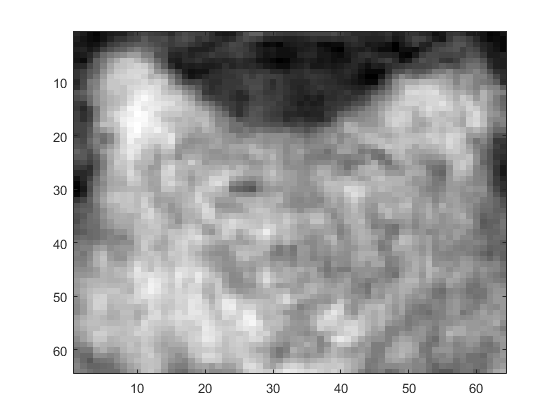
\includegraphics[scale=.4]{w_cat.png}
\caption{The projection of the first cat onto the basis of dogs.}
\end{center}
\end{figure}

Then I used the followingto find the orthogonal complement. 

\begin{align*}
w_{cat}^\perp &= C_1-w_{cat}\\
w_{dog}^\perp &= D_1-w_{dog}.
\end{align*}

Then the code followed immediately.

\begin{lstlisting}
%calculate w_perp_cat by w_perp_cat = C(:,1)-w_cat
w_perp_cat = C(:,1) - w_cat;
%Plot w_perp_cat
imagesc(reshape(w_perp_cat(:,1),64,64))
\end{lstlisting}

\begin{figure}[h]
\begin{center}
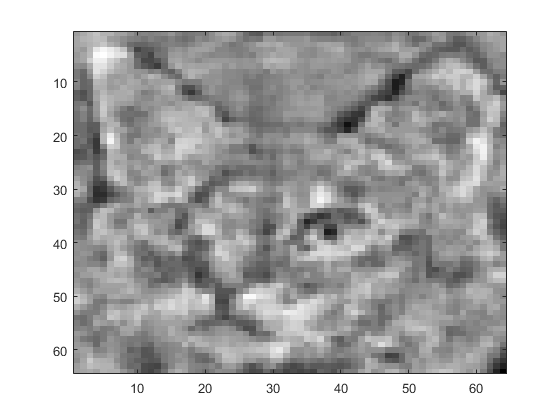
\includegraphics[scale=.4]{w_perp_cat.png}
\caption{The orthogonal complement of the previous vector.}
\end{center}
\end{figure}

\pagebreak

%%%%%%%%%%%%%%%%%%%%%%%%%%%%%%%%%%%%%%%%%%%%%%%%%%%%%%%%%%%%%%%%%%%%%%%%%%%%%%%%%%%%%%%%%%%%%%%%%%%%%%%%%%%%%%%%%%%%%
%%%%%%%%%%%%%%%%%%%%%%%%%PROBLEM%%%%%%%%%%%%%%%%%%%%%%%%%%%%%%%%%%%%%%%%%%%%%%%%%%%%%%%%%%%%%%%%%%%%%%%%%%%%%%%%%%%%%%%%%%%%%%%%%%%%%%%%%%%%%%%%%%%%%%%%%%%%%%%%%%%%%%%%%%%%%%%%%%%%%%%%%%%%%%%%%%%%%%%%%%%%%%%%%%%%%%%%%%%%%%%%%%%%%%%%%%


\noindent\textbf{Problem 3.} \\
I explained the methodology in the previous problem and in this case we just have dog vectors instead of cat. The code and images follow.

\begin{lstlisting}
%Create a w_dog vector and w_dog_perp
w_dog = zeros(4096,1);
w_perp_dog = zeros(4096,1);
%Make a for loop to calculate each component of the w_dog vector
for i=1:99
    w_dog(:,1) = dot(D(:,1),U_cat(:,i))*U_cat(:,i)+w_dog(:,1);
end
%Plot w_dog
imagesc(reshape(w_dog(:,1),64,64))
\end{lstlisting}

\begin{figure}[h]
\begin{center}
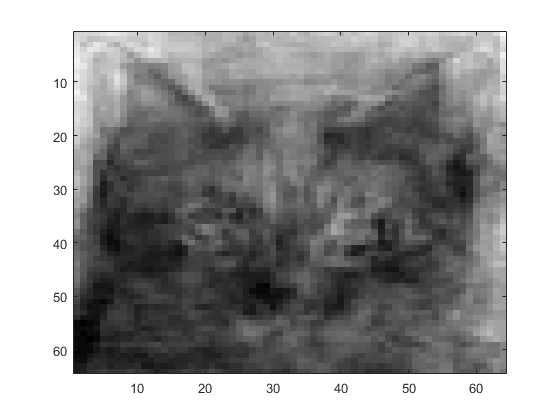
\includegraphics[scale=.4]{w_dog.png}
\caption{The projection of the first dog onto the basis of cats.}
\end{center}
\end{figure}

Then I used the following to find the orthogonal complement.

\begin{lstlisting}
%calculate w_perp_dog by w_perp_dog = D(:,1)-w_dog
w_perp_dog = D(:,1) - w_dog;
%Plot w_perp_dog
imagesc(reshape(w_perp_dog(:,1),64,64))
\end{lstlisting}

\begin{figure}[h]
\begin{center}
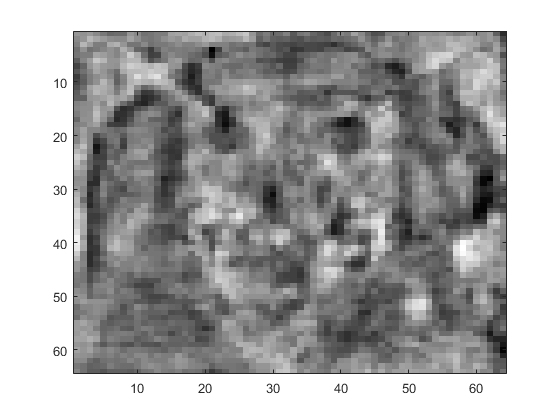
\includegraphics[scale=.4]{w_perp_dog.png}
\caption{The orthogonal complement of the previous vector.}
\end{center}
\end{figure}

\pagebreak


%%%%%%%%%%%%%%%%%%%%%%%%%%%%%%%%%%%%%%%%%%%%%%%%%%%%%%%%%%%%%%%%%%%%%%%%%%%%%%%%%%%%%%%%%%%%%%%%%%%%%%%%%%%%%%%%%%%%%
%%%%%%%%%%%%%%%%%%%%%%%%%PROBLEM%%%%%%%%%%%%%%%%%%%%%%%%%%%%%%%%%%%%%%%%%%%%%%%%%%%%%%%%%%%%%%%%%%%%%%%%%%%%%%%%%%%%%%%%%%%%%%%%%%%%%%%%%%%%%%%%%%%%%%%%%%%%%%%%%%%%%%%%%%%%%%%%%%%%%%%%%%%%%%%%%%%%%%%%%%%%%%%%%%%%%%%%%%%%%%%%%%%%%%%%%%


\noindent\textbf{Problem 4.} \\
First, we calculate $\|u\|^2$ by just calculating $\langle u,u\rangle$.  In this case we let $u=C_1$, the first cat picture which corresponds to the first column of the cat $C$ matrix.  This is what we will compare to $T_k(u)$.  To find $T_k(u)$ we merely calculate
\begin{align*}
T_k(u)=\sum_{i=1}^k \langle u, U_{{cat}_i} \rangle U_{{cat}_i}.
\end{align*}
Then, I create a vector where the $k$th entry is given by $\langle T_k(u),T_k(U)\rangle=\|T_k(u)\|^2$. After finding the whole vector, I take the square root of each entry and compare it to $\|u\|$.  Here I made a plot of $\|T(u)\|$ which I then plotted along with $\|u\|$ to make a direct comparison.  This comparison verifies $\|T(u)\|\leq \|u\|$. Here is the code snippet:

\begin{lstlisting}
%Create a matrix of values for the ||Tu||_2^2 for varying k
Tu_norm_vec = zeros(99,1);
inprod_k = 0;
norm_Tu_square = 0;
norm_u_square=dot(C(:,1),C(:,1));
for k=1:99
    inprod_k = dot(C(:,1),U_cat(:,k));
    norm_Tu_square = inprod_k^2+norm_Tu_square;
    Tu_norm_vec(k,1)=norm_Tu_square;
end
%Make a vector of values all ||u||^2 to compare to ||Tu||^2
norm_u_vec = zeros(99,1);
for k=1:99
    norm_u_vec(k,1) = norm_u_square;
end
%And make a vector for "x" values
x=zeros(99,1);
for k=1:99
    x(k,1) = k;
end
%Now plot the square roots of what I found before!
plot(x,sqrt(Tu_norm_vec(:,1)),x,sqrt(norm_u_vec))
\end{lstlisting}

\begin{figure}[h]
\begin{center}
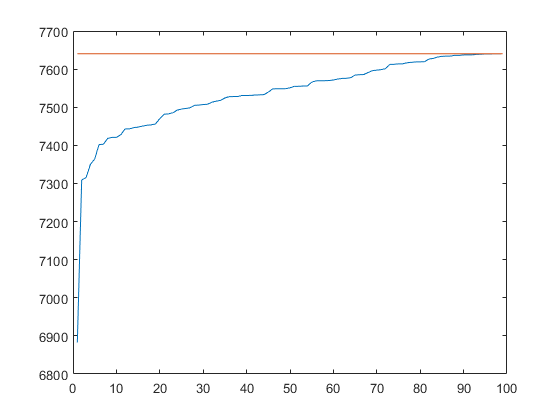
\includegraphics[scale=.4]{norm_tu.png}
\caption{Comparing $\|T(u)\|$ (blue) to $\|u\|$ (red).}
\end{center}
\end{figure}

\pagebreak





%%%%%%%%%%%%%%%%%%%%%%%%%%%%%%%%%%%%%%%%%%%%%%%%%%%%%%%%%%%%%%%%%%%%%%%%%%%%%%%%%%%%%%%%%%%%%%%%%%%%%%%%%%%%%%%%%%%%%
%%%%%%%%%%%%%%%%%%%%%%%%%PROBLEM%%%%%%%%%%%%%%%%%%%%%%%%%%%%%%%%%%%%%%%%%%%%%%%%%%%%%%%%%%%%%%%%%%%%%%%%%%%%%%%%%%%%%%%%%%%%%%%%%%%%%%%%%%%%%%%%%%%%%%%%%%%%%%%%%%%%%%%%%%%%%%%%%%%%%%%%%%%%%%%%%%%%%%%%%%%%%%%%%%%%%%%%%%%%%%%%%%%%%%%%%%


\noindent\textbf{Problem 5.} \\
Here we find that the largest eigenvalue is the square of the largest singular value found from the previous exercise. It's worth noting that the largest eigenvalue corresponds to the last diagonal entry, and thus the principal component is the last column in the matrix of eigenvectors.  I checked this and found the image via the following.

\begin{lstlisting}
%Compute CC^T
mat_C = C*transpose(C);
%Find eigenvalues and vectors of CC^T
[V_c,D_c] = eig(mat_C);
%Display the eigenvector with largest eigenvalue
imagesc(reshape(V_c(:,4096),64,64))
%What is the largest eigenvalue?
largest_eval = D_c(4096,4096)
%Compare to the largest singular value
largest_singval = S_cat(1,1)
%Square this
largest_singval_square = largest_singval^2
\end{lstlisting}

\begin{figure}[h]
\begin{center}
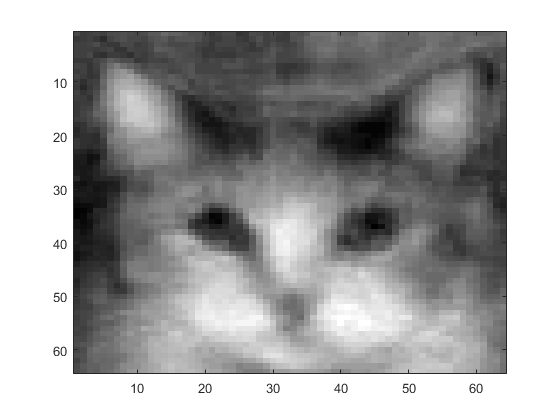
\includegraphics[scale=.4]{evector.png}
\caption{The eigencat corresponding to the largest eigenvalue.}
\end{center}
\end{figure}


\end{document}

